% A core aspect of human intelligence is adapting to new tasks quickly while drawing upon relevant past learning experiences. 
Meta-learning~\citep{schmidhuber1987, Naik1992MetaneuralNT,santoro2016meta, vinyals2016matching, finn2017model} can achieve quick adaption for UNSEEN tasks by identifying common structures among various SEEN tasks, enabling faster learning of a new task with as little data as possible. 
However, existing meta-learning techniques (\emph{e.g.,} MAML~\citep{finn2017model}) often fail to generalize well when the test tasks belong to a different distribution from the training tasks distribution~\citep{Chen2019ICLR}. 
% For example, MAML assumes equal weights to all samples in the same task and equal weights to all tasks in the training task distribution during meta-training.
For example, MAML assumes equal weights to all samples and tasks during meta-training.
This task homogeneity assumption of MAML often limits its ability to work in real-world applications. 
\begin{figure}[!t]
%\captionsetup[subfigure]{aboveskip=-2pt,belowskip=-2pt}
    \centering
    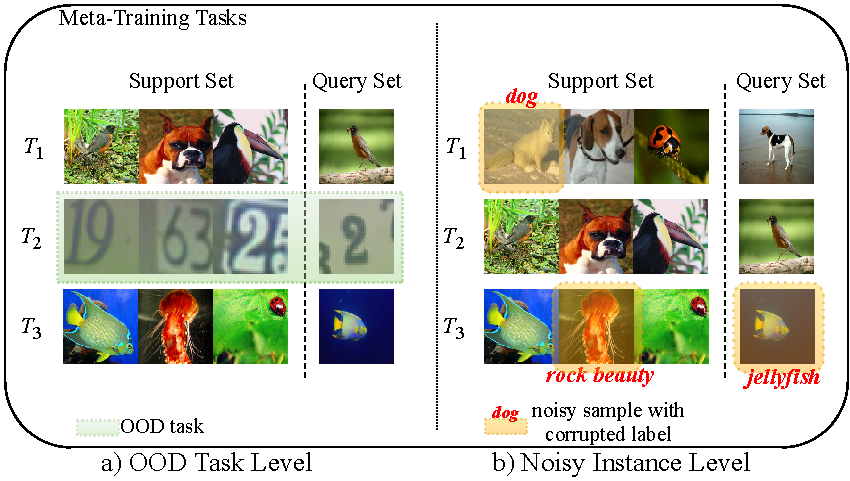
\includegraphics[width=0.47\textwidth, height=4.2cm]{figs/outliers.pdf}
    \vspace{-7mm}
    \caption{We consider corrupted training set for few-shot learning in this work: a) OOD task level and b) noisy instance level. $T_2$ in a) is an OOD task that is sampled from a different distribution. b) contains some noisy samples which are mislabeled. For example, the actual label of the first sample in $T_1$ should be ``\textit{Arctic fox}" which is labeled as ``\textit{dog}"; The labels of two noisy samples in $T_3$ are flipped wrongly. The first one should be ``\textit{rock beauty}," and the other one should be ``\textit{jellyfish}."}
    % {Solid green squares and circles represent tasks sampled from the in-distribution dataset (\textit{e.g.,} \textit{mini}-ImageNet~\citep{ravi2016optimization}); red triangles indicate tasks sampled from out-of-distribution (OOD) dataset (\textit{e.g.,} SVHN~\citep{netzer2011reading}). Training and testing domains (a) are subsets of the data domain; (b) have some overlap between each other where some OOD tasks (\textit{e.g.} $30\%$, etc.) are involved in the training domain; \textbf{We consider type (b) in our paper}.}
    \label{fig:motivation}
\vspace{-8mm}
\end{figure}

\begin{figure*}[!htbp]
%\captionsetup[subfigure]{aboveskip=-2pt,belowskip=-2pt}
    \centering
    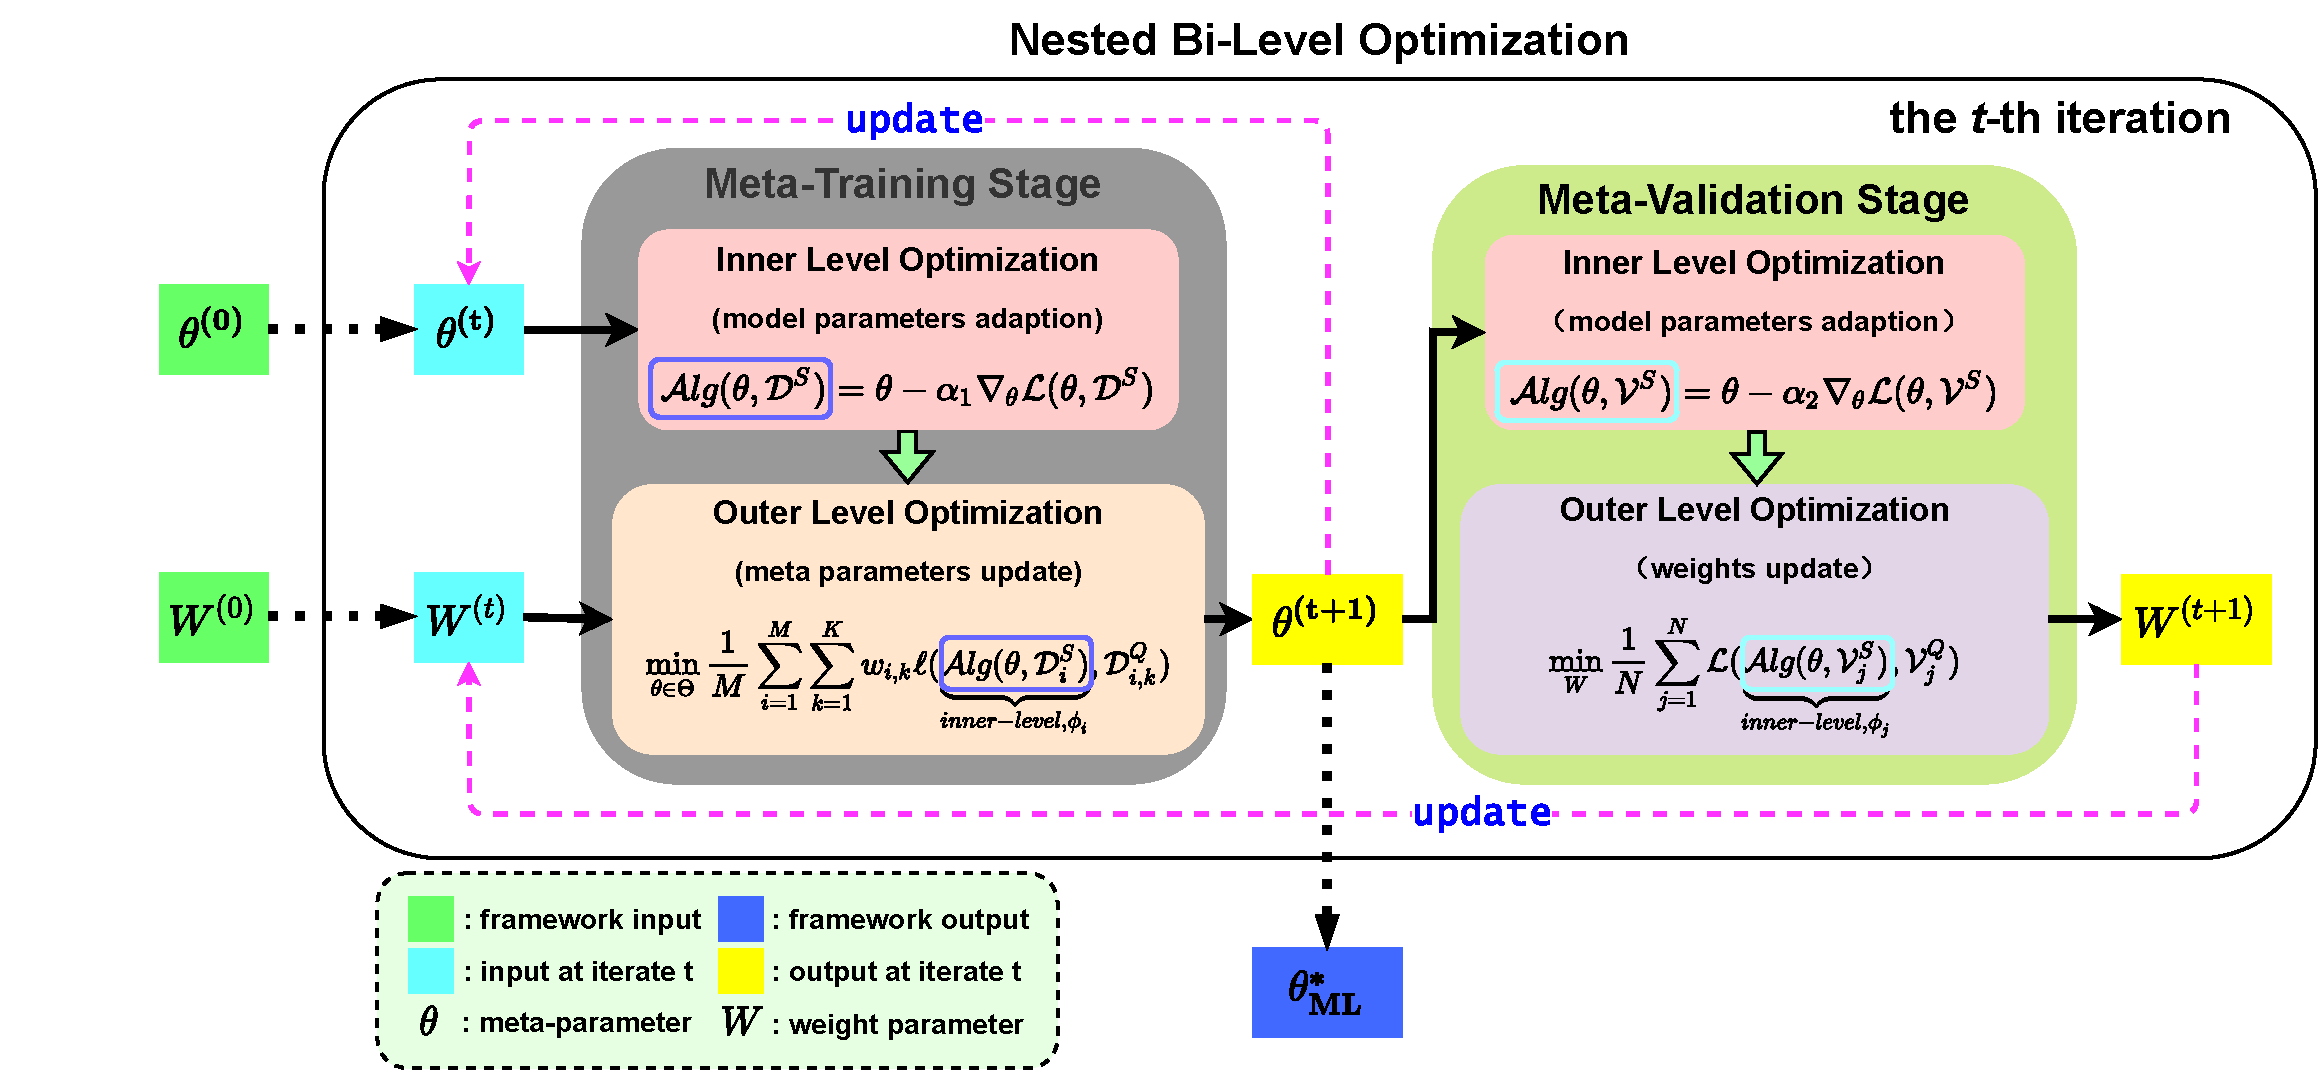
\includegraphics[width=0.85\linewidth, height=6.5cm]{figs/overview.pdf}
    \caption{Overview of our \sysname{} framework that solves a \textit{\biopt{}} optimization problem. (a) In the meta-training stage, model parameters $\phi_i$ of each task are adapted from meta-parameter $\boldsymbol{\theta}$ through the inner level optimization; (b) In the outer-level of the meta-training stage, we update the meta-parameters using the weights $W$ from the previous iterate; (c) Weights are further updated in the meta-validation stage using the gradient of the meta-losses with respect to current $W$.} 
    \label{fig:overview}
    \vspace{-4mm}
\end{figure*}

We motivate the importance of robust meta-learning when meta-training tasks have OOD tasks using the following examples. For example, consider the task of detecting vehicles at night under different weather conditions. In this case, the meta-test tasks only consist of images of vehicles at night. Since the procurement vehicles driving data at night, covering all critical scenarios is difficult, we need a model that can quickly adapt to rare driving conditions. Hence, we consider meta-training tasks to consist of images of the vehicles in multiple lighting scenarios. In this case, some of the tasks in meta-training may degrade the meta-test performance. So, it is vital to have a meta-learning model that is robust to OODs.

Another example is rare lung cancer detection from medical x-ray images. Since the procurement of rare lung cancer images is both problematic and expensive, it is beneficial to use prior knowledge of cancer images. Specifically, the meta-test tasks contain images of rare lung cancer, whereas meta-training tasks consist of general cancer x-ray images. In the examples given above, meta-test tasks belong to specialized slices where the data availability is meager compared to meta-training tasks. The meta-training task distribution is biased compared to that in the meta-test. To keep the whole meta-training tasks for generalization and reduce the adverse impact of the biased distribution in meta-training, we propose a novel robust few-shot learning algorithm in the presence of outliers in meta-training time, which is similar to the corruptions in training time in the traditional robust learning~\citep{schneider2020improving}. This is different from the existing robust few-shot learning papers~\cite{yin2018adversarial, lu2020robust, goldblum2020adversarially} which consider the corruption only happens in meta-test time.     

To simulate the corruptions in meta-training, two levels of outliers (Figure \ref{fig:motivation}) are considered: {\textit{a}}) Out-Of-Distribution (OOD) task, where the meta-training has tasks that are out of distribution to the meta-test tasks (i.e., the meta-test dataset is a specialized slice of meta-train) and {\textit{b}}) noisy instance level, where some of the labels might be noisy (due to human labeling errors or inherent ambiguity of certain classification problems) for meta-training samples. 

A natural way of dealing with corrupted data in meta-training is by assigning weights to either tasks or individual instances. For example, assigning zero weight to OOD or noisy tasks/instances in the meta-train set improves the meta-learning algorithm's performance. Inspired by~\citep{ren2018learning}, in this work, we propose an end-to-end robust meta-learning framework called \sysname{} that can achieve the reweighting schema along with learning good model initialization parameters in the few-shot learning scenario.  

% The resulting problem is an extension of meta-learning called \emph{weighted meta-learning}. Weighted meta-learning has been studied in~\citet{cai2020weightedmeta}, where they study the weighting on a restricted class of loss functions like the square loss and hinge loss. 


%An efficient meta-learning algorithm should learn the corresponding meta-knowledge of vehicle detection or tumor detection useful for faster learning of specialized tasks like detecting vehicles at night or rare cancer.

% \vspace{-1ex}
% \subsection{Our Contributions}
% Our work's significant contribution is introducing the nested MAML (\sysname{}) algorithm, an end-to-end framework for the reweighted MAML training. 

\sysname{} considers the weights as hyper-parameters and uses a small set of meta-validation tasks representing the meta-test tasks to find the optimal hyper-parameters by minimizing the meta-loss on the validation tasks in a \textbf{\biopt{}} manner.  An overview of \sysname{} is given in Figure \ref{fig:overview}. In practice, the size of the meta-validation tasks set required by \sysname{} is tiny compared to the meta-training dataset. Hence, creating a  small and clean meta-validation set is neither expensive nor unrealistic, even for rare specialized use cases of a real-life scenario. A similar strategy has been applied in ~\citep{ren2018learning,shu2019meta,killamsetty2020glister}. However, they focus on traditional supervised learning, and we generalize this to task- and instance-level in a meta-learning setting. Since \sysname{} uses an online framework to perform a joint optimization of the weight hyper-parameters and model parameters for the weighted MAML model, the computational time of ours is comparable to MAML.
% specifically 1.5 times MAML's running time. %Finally, we compare \sysname{}'s performance to existing robust meta-learning and hyperparameter optimization algorithms through extensive experiments on real-world and synthetic datasets for {\textcolor{red}{out-of-distribution (OOD), noisy-labels settings in training data}}.

\noindent \textbf{Contributions of our work are summarized as follows:} 1) We study the general form of the task and instance weighted meta-learning, where we learn the optimal weights and model initialization parameters by optimizing a \textit{\biopt{}} objective function. To the best of our knowledge, ours is the first work that studies the \textit{\biopt{}} optimization problem, which comes naturally in such a new setting. 2) We introduce a novel algorithmic framework \sysname{} that uses a small set of validation tasks to enable robust meta-learning. We solve the \emph{\biopt{}} optimization problem efficiently through a series of practical approximations and provide a theoretical convergence analysis for \sysname{}. In particular, we show that \sysname{} converges in $\mathcal{O}(1/\epsilon^2)$ iterations under reasonable assumptions and contrast this with existing bounds of MAML. 3) We provide comprehensive synthetic and real-world data experiments demonstrating that \sysname{} achieves state-of-the-art results in two scenarios (OOD tasks and noisy instance labels).

\vspace{-1ex}
\section{Related Work}
% \textbf{Meta Learning.} 
% \vspace{-1ex}
There are several lines of meta-learning algorithms: nearest neighbors-based methods~\citep{vinyals2016matching}, recurrent network-based methods~\citep{ravi2016optimization}, and gradient-based methods. As the representative of gradient-based meta-learning algorithms, MAML~\citep{finn2017model} and its variants ~\citep{finn2018probabilistic, nichol2018first, rusu2018meta,rajeswaran2019meta, behl2019alpha, raghu2019rapid, zhao2020fair, zhou2020meta} learn a shared initialization of model parameters across a variety of tasks during the meta-training phase that can adapt to new tasks using a few gradient steps.~\citet{cai2020weightedmeta} proposes a simple weighted meta-learning approach only for the basis regression problem that selects weights by minimizing a data-dependent bound involving an empirical integral probability metric between the weighted sources and target risks. However, this approach cannot be easily extended to complex scenarios with arbitrary loss functions.
% In contrast, \sysname{} can handle arbitrary loss functions.
% and \textit{b}) jointly learn the weights along with the meta-learning model parameters.  % Our \sysname{} algorithm poses the weights as hyper-parameters of the model and tries to estimate these weights by minimizing the nested loss over the model parameters and weight hyper-parameters. \sysname{} can be applied to any loss functions at the expense of the computational costs due to the need for higher-order differentiation in the computation graph.
% ~\cite{yao2020automated} proposes ARML, which extracts the cross-task relations and constructs the meta-knowledge graph to enable the model to find a specific meta learner for the new task.

% \noindent \textbf{Learning with OOD tasks.} %Because of task homogeneity assumption limitation, MAML does not perform well on the training tasks sampled from different distributions ~\citep{vuorio2019multimodal}. 
There are few meta-learning papers discussing learning with OOD tasks. ~\citet{jeong2020ood} propose an OOD detection framework in meta-learning through generating fake samples which resemble in-distribution samples and combine them with real samples. However, they assume the outlier instances exist in the query set, which is different from ours. The most relevant field is from the perspective of task heterogeneity~\citep{vuorio2019multimodal, triantafillou2019meta,yao2020automated}. ~\citet{vuorio2019multimodal} proposed  MMAML to deal with multimodal task distribution with disjoint and far apart modes and generates a set of separate meta-learned prior parameters to deal with each mode of a multimodal distribution. If we view that all the OOD tasks belong to a single mode, this is relevant to our setting. To tackle the distribution drift from meta-training to meta-test, B-TAML~\citep{lee2020l2b} learn to relocate the initial parameters to a new start point based on the arriving unseen tasks in the meta-test. The setting considered in our work and B-TAML work can be viewed as similar if we assume some of the datasets considered in the multi-dataset classification setting of B-TAML as OOD datasets.
%Among the meta-training tasks, some tasks are Out-of-Distribution (OOD) if they have a very different distribution from others. 

% \noindent \textbf{Learning with noisy labels.} 
To tackle samples with corrupted labels, some researches~\citep{luo2015foveation, jalal2017robust, wang2019direct} introduce noise-robust models.~\citet{ren2018learning} and~\citet{shu2019meta} propose a noisy data filtering strategy using an instance reweighting strategy where the weights are learned automatically. However, the effect of noisy labels on few-shot learning requires more attention. Although ~\citep{yin2018adversarial,lu2020robust,goldblum2020adversarially} proposes robust meta-learning or few-shot learning, they assume a presence of outliers containing in meta-test, which is different from ours. 
% In contrast, \sysname{} does not require any additional information about noisy samples in its learning.}%to deal with the training tasks containing data instances with noisy labels. 

% In contrast, ~\citep{han2018co, chen2019understanding}propose noisy data filtering techniques to reduce noisy labels' impact. 
%Our paper is the first to consider the training tasks with noisy labels without any additional information about noisy samples in the few-shot learning framework to the best of our knowledge. 

%for noise filtering that solves a bi-level optimization problem on instance weights. In contrast~\cite{shu2019meta} uses an MLP as a weighting function, explicitly mapping sample weights adaptively from the data. 
%Many researchers focus on learning with noisy labels to avoid extravagant relabeling costs by improving deep learning models' robustness.
% ~\cite{han2018co} proposes a co-teaching model that trains two neural networks simultaneously, and they will teach each other to detect noisy samples. INCV~\citep{chen2019understanding} applies cross-validation to randomly split noisy datasets and use the selected samples to train the model. ~\cite{ren2018learning} proposes a gradient-based method to assign weights to training samples by online meta-learning strategy.
% For comparison, we consider two baselines that use Co-teaching~\citep{han2018co} and INCV~\citep{chen2019understanding} to clean noisy datasets first and apply MAML to the selected data.